\documentclass[12pt]{article}
\usepackage[utf8]{inputenc}
\usepackage{array}
\usepackage{xcolor}
\usepackage{graphicx}
\usepackage{mathtools}
\usepackage{amsmath}
\usepackage{multicol}
\usepackage{eqnarray}
\usepackage{wrapfig}


\usepackage{natbib}
\usepackage{hyperref}
\hypersetup{
	colorlinks=true,
	linkcolor=black,
	filecolor=mangeta,      
	urlcolor=blue,
	pdftitle={Overleaf Example},
	pdfpagemode=FullScreen,
}

\usepackage[margin=0.6in]{geometry}

\title{52nd—24th INTERNATIONAL-RUDOLF ORTVAY \\ PROBLEM SOLVING CONTEST IN PHYSICS \\ Problem 4}
\author{Nguyen Thanh Long}
\date{\today}

\begin{document}
	
\maketitle
	
a) The time that a body need to soar and turn back to the horizontal plane is $T = \frac{2v}{g}$ where $v$ is the initial vertical velocity of that body.

In this problem, we call $v_x$ and $v_y$ are the initial horizontal velocity and the initial vertical velocity of the ball. After hiting the wall, the ball will have the horizontal velocity is $k v_x$. So time for the ball hit the wall will be $k$ times to bounce back $A$. So that, we have:
$$ \frac{v_y}{g} = k \left( \frac{v_y}{g} + 2k \frac{v_y}{g} + 2 k^2 \frac{v_y}{g} + 2 k^3 \frac{v_y}{g} + ... + 2 k^N \frac{v_y}{g} \right) $$
$$ \Leftrightarrow 1 = k \left( 2 \frac{1 - k^{N+1}}{1 - k} - 1 \right) .$$
$$ \Leftrightarrow N = \log_k \left( \frac{k^2 + 2k - 1}{2} \right) - 2 .$$

Choose $f(x) = \log_x \left( \frac{x^2 + 2x - 1}{2} \right) -2$ with $x<1$ and $f^{-1}(x)$ is the inverse function of $f(x)$. 

\begin{figure}[!htb]
	\centering
	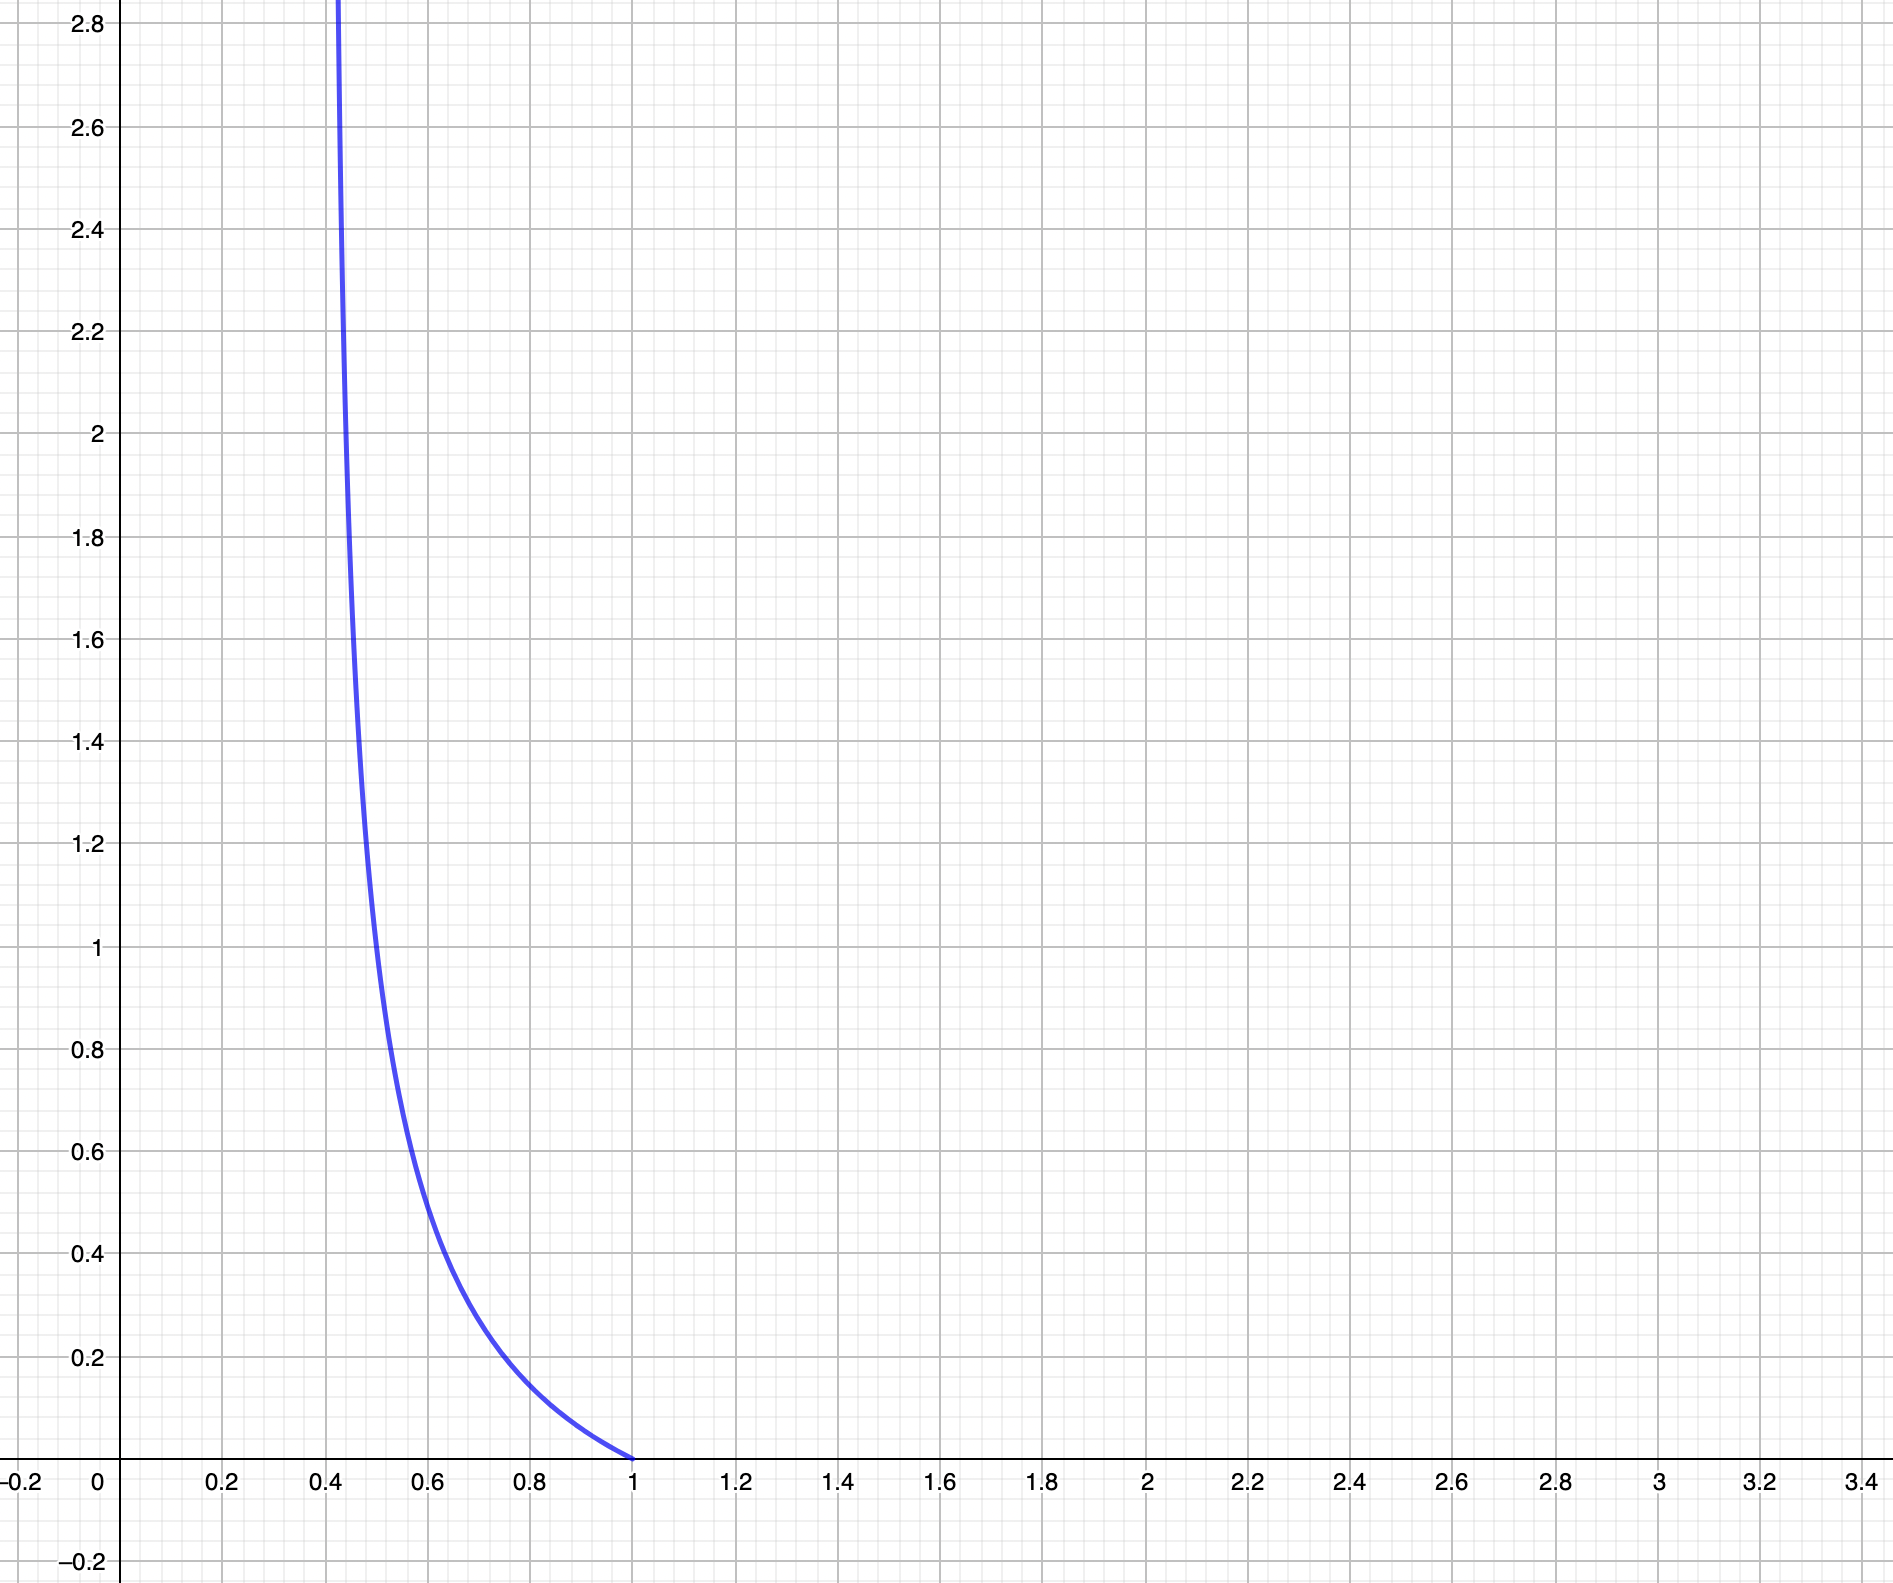
\includegraphics[width=0.5\textwidth]{Fig P4.png}
	\caption{ Function $y=f(x)$ }
\end{figure}	

So we can write:
$$k = f^{-1}(N).$$

When $N \rightarrow \infty$, $k \rightarrow -1 + \sqrt{2} \approx 0.414 $ and when $N=1$, $k= \frac{1}{2}$. \\

b) Cause the time the ball in the air only depend on $v_y$ and $k$, so we let $v_y=v$. This time is:
$$ t = 2\frac{v}{g} + 2k \frac{v}{g} + 2 k^2 \frac{v}{g} + 2 k^3 \frac{v}{g} + ... = \frac{2v}{g ( 1 - k )}  .$$

When $N= \infty$, time the ball in the air is $t= \left( 2 +\sqrt{2} \right) \frac{v}{g} \approx 3.414 \frac{v}{g} .$
	
\end{document}